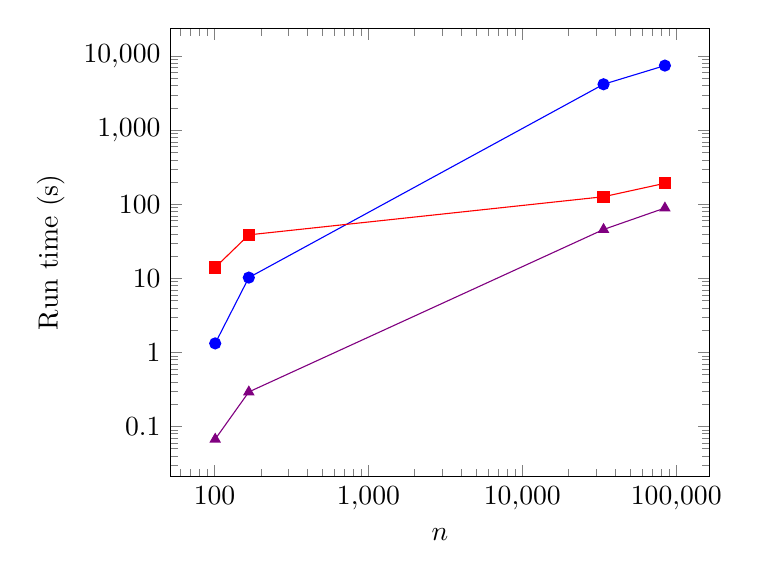
\begin{tikzpicture}
    \begin{loglogaxis}[xlabel=$n$,
			ylabel=Run time (s),
			log ticks with fixed point,]
      % [width=\linewidth,
      %            height=4cm, enlarge y limits=.2,
      %            ytick={1, 2}] % , yticklabels={Wrong, Right}
      %\addplot+ [boxplot={whisker range=\boxplotbignum}] table [y index=0] {figures/data.1.txt};
      % Ignore the miscalculations here
      %\addplot+ [boxplot prepared={draw position=2,
      %                             median=662,
      %                             lower whisker=222,
      %                             upper whisker=1558,
      %                             upper quartile=867,
      %                             lower quartile=478.5}] coordinates {};
	%% 
	%% Runtime for computing k number of graphs as a function of datasets' number of nodes
	%%
  %	EMAIL CORE
  %	RADOSLAW
	%	enron (full)
	%	email-Enron.txt
  %% PHRG
    \addplot[color=blue,mark=*] table [col sep=comma]
			{
      101, 1.32355809212
      167, 10.2496099472
			33696, 4188.344877
      84384, 7487.98321414
      };
    %% CHLU
    \addplot[color=violet,mark=triangle*] table [col sep=comma]
    	{
      101, 0.0673129558563
      167, 0.292577981949
			33696, 45.7626059055
      84384, 89.1664869785
      };

    %% KRON
    \addplot[color=red,mark=square*] table [col sep=comma]
			{
			101, 14.0635240078
      167, 38.7150030136
			33696, 126.776366949
      84384, 192.528311968
			};
    \end{loglogaxis}
\end{tikzpicture}
